\documentclass[handout]{beamer} 
  \usetheme{Warsaw}
  \usepackage{graphicx}
  \setbeamercovered{transparent}
  \setbeamerfont{footnote}{size=\tiny}
  \usepackage{pgfplots}
  \usepackage[backend=biber, maxbibnames=9, maxcitenames=9,style=alphabetic, sorting=ynt]{biblatex}
  \addbibresource{references.bib}
  \usepackage{microtype}
  \usepackage{parskip}
  \setlength{\parindent}{0pt}
  \usepackage{adjustbox}

  \renewcommand{\bibfont}{\normalfont\tiny}

  \theoremstyle{plain}
  \newtheorem{question}{Question}

  % personal pref: serif for math and sans for text. I'm willing to possibly change this if it's disliked. --Nat
  \usefonttheme[onlymath]{serif}

  \begin{document}

  \title{Unfolding orthogonal polyhedra}
  \subtitle{A survey of previous works}
  \author{Natalie Stewart}
  \date{Dec 1, 2020}
  \frame{\titlepage}



  \begin{frame}{Review of orthogonal polyhedra}
    \begin{columns}
      \begin{column}{0.8\textwidth}
        \begin{itemize}
          \item A polyhedron is \emph{orthogonal} if its faces are:
            \begin{enumerate}
              \pause \item \emph{orthogonal to each other} and 
              \pause \item \emph{each perpendicular to the $x$, $y$, or $z$ axis.}
            \end{enumerate}
            \pause Abuse of notation: a polyhedron ``is'' its bounding surface.
          \pause \item The \emph{genus} of an connected orientable closed surface is one of the following equivalent data:
            \begin{itemize}
              \item The number of ``handles'' it has.
              \item The maximum number of cuttings along non-intersecting simple closed curves without disconnecting the surface.
              \item $1 - \frac{\chi}{2}$, where $\chi$ is the \emph{Euler characteristic}.
            \end{itemize}
        \end{itemize}  
      \end{column}
      \begin{column}{.2\textwidth}
        \begin{center}
          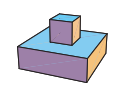
\includegraphics[width=.8\textwidth]{./figs/genus_0_orthogonal_polyhedron.png}\\
          \tiny\textbf{Figure}: a genus 0 orthogonal polyhedron.\footnote[frame]{\fullcite[Fig. 22.4]{Demaine_textbook}}\\
          \; \\
          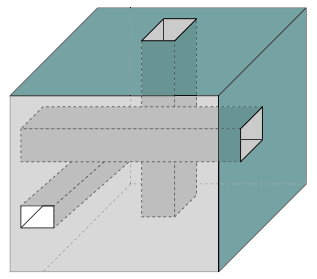
\includegraphics[width=.8\textwidth]{./figs/genus_3_orthogonal_polyhedron.png}\\
          \tiny\textbf{Figure}: a genus 3 orthogonal polyhedron.\footnote[frame]{\fullcite[Fig. 7]{Damian_Demaine}}
        \end{center}
      \end{column}
    \end{columns}
  \end{frame}

  \begin{frame}{Review of unfolding}
    \begin{itemize}
      \item An \emph{unfolding} of a surface is an isometry between it and a simple polygon.
      \pause \item An \emph{edge unfolding} of a polyhedron is an unfolding of a cut of a polyhedron along edges.
      \pause \item Some orthogonal polyhedra have no edge unfoldings!
        To find more unfoldings, we need to relax the constraints\ldots 
    \end{itemize}
  \end{frame}

  \begin{frame}{Review of unfolding 2}
    \begin{itemize}
      \item A \emph{grid with $k \times k'$ refinement} on an orthogonal polyhedron is the graph formed by adding edges given by the intersection of the surface with planes along each face, then replacing each non-split rectangle with a $k \times k'$ grid of rectangles.
      \pause \item A \emph{grid unfolding of an orthogonal polyhedron with $k \times k'$ refinement} is an edge unfolding of the polyhedron with edges corresponding with a grid with $k \times k'$ refinement. 
    \end{itemize}
    \begin{center}
    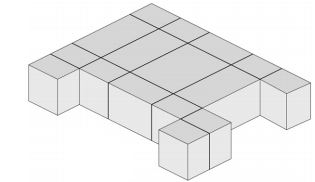
\includegraphics[width=.3\textwidth]{./figs/grid.png}
    \hspace{.1\textwidth}
    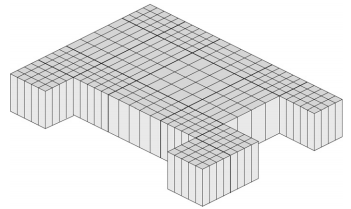
\includegraphics[width=.3\textwidth]{./figs/refined_grid.png}\\
    \tiny\textbf{Figure}: on the left is a grid. On the right is a grid with $5 \times 4$ refinement.\footfullcite[Fig. 4]{Damian_Flatland_Orourke}
    \end{center}
  \end{frame}

  \begin{frame}{The central problem}
    \begin{question}
      What is the smallest $k,k'$ such that every orthogonal polyhedron has a grid unfolding with $k \times k'$ refinement?
    \end{question}
    \pause Here is a summary of many special cases of $k,k'$ we know to work;
    don't sweat terminology you don't know.
    \adjustbox{max width=\textwidth}{  
      \begin{tabular}{|c | c | c| c|}
        \hline
        Class & Refinement & Reference\\
        \hline
        \hline
        Orthogonal polyhedra & Open &  \\ 
        Genus $g \leq 2$ orthogonal polyhedra & $O(n) \times O(n)$ & \cite{Chang_Yen,Damian_Demaine} \\
        \hline
        Genus $g$ one-layer polyhedra & $2 \times 1$ on only $2(g-1)$ faces & \cite{Chang_Yen} \\
        \hline
        Well-separated orthographs & $2 \times 1$ & \cite{Ho_Chang_Yen} \\
        Orthotrees & $4 \times 4$ & \cite{Damian_Flatland,Damian_Flatland_Better} \\
        Orthotubes & $1 \times 1$ & \cite{Biedl_Demaine} \\
        Orthostacks & $2 \times 1$ & \cite{Biedl_Demaine} \\
        Manhattan towers & $5 \times 4$ & \cite{Damian_Flatland_Orourke_Manhattan} \\
        \hline
        Regular orthogonal polyhedra w/ $x-$ and $z-$holes & $2 \times 1$ & \cite{Ho_Chang_Yen} \\
        \hline
      \end{tabular}}
      \pause We'll focus mostly on the genus $g = 0$ case.
  \end{frame}

  \begin{frame}{References for ``the chart''}
    \printbibliography
  \end{frame}

  \begin{frame}{Structure of the talk}
    We'll follow the following structure
    \begin{enumerate}
      \item Review terminology around unfoldings,
      \pause \item Review the epsilon-unfolding algorithm for grid-unfolding genus 0 orthogonal polyhedra with exponential refinement.
      \pause \item Introduce delta-unfolding algorithm for the genus $0$ case with quadratic refinement. 
      \pause \item Introduce the linear unfolding algorithm for the genus 0 case with linear refinement.
      \pause \item Sketch the extension of the linear unfolding algorithm to genus $g \leq 2$ polyhedra.
    \end{enumerate}
  \end{frame}

  \begin{frame}{Review: layers, bands, unfolding trees, rims}
    We'll review terminology from the \emph{epsilon unfolding strategy} due to Damian, Flatland, and O'Rourke \footfullcite{Damian_Flatland_Orourke}:
    \begin{itemize}
      \pause \item $xz$ faces extend to planes slicing the polyhedron into \emph{layers}.
      \pause \item Each layer is made of $xz$ faces conneccting cylindrical \emph{bands}.
      \pause \item Suppose we have genus $g = 0$.
        Then, bands are the vertices in an \emph{unfolding tree}, where adjacencies are determined by \emph{$z$-beams}.
      \pause \item Arbitrary choice of \emph{root node} having one rim circling a simply connected face yields a directed unfolding tree.
      \pause \item Bands are bounded by circular \emph{rims}; the \emph{front rim} connects to a parent (if one exists) and the other is the \emph{back rim}.
    \end{itemize}
  \end{frame}

  \begin{frame}{Illustration of layers and bands}
    \begin{center}
      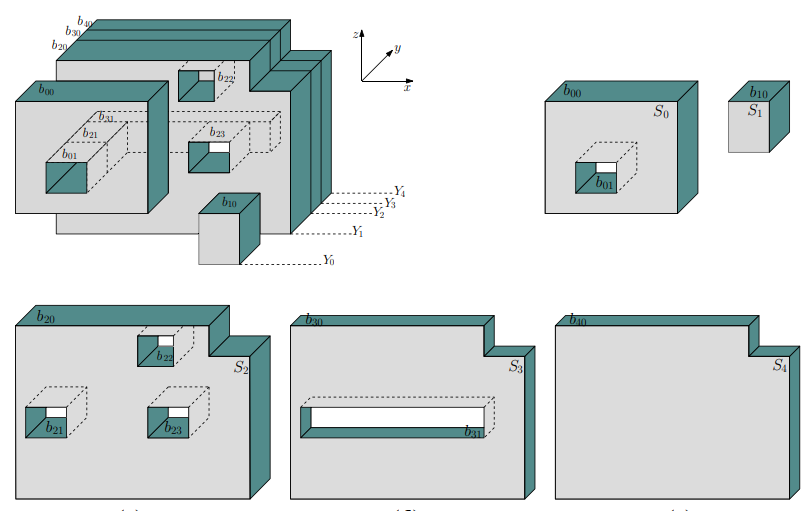
\includegraphics[width=.9\textwidth]{./figs/Layer_decomposition.png}\\
      \tiny \textbf{Figure}: a decomposition of an orthogonal polyhedron of genus 1 into layers.
      \footfullcite[Fig. 1]{Damian_Demaine}
    \end{center}
  \end{frame}

  \begin{frame}{Illustration of an unfolding tree} 
    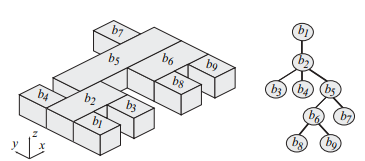
\includegraphics[width=\textwidth]{./figs/Unfolding_tree.png}
    \begin{center}
      \footnotesize \textbf{Figure}: a particularly simple orthogonal polyhedron and an unfolding tree. \footfullcite[Fig. 2]{Damian_Flatland_Orourke}
    \end{center}
  \end{frame}

  \begin{frame}{Meta-outline of the strategy}
    We recursively construct a \emph{spiral path} which:
    \begin{itemize}
      \item begins and ends at the front rim of the root node,
      \pause \item spirals around each band at least once, and
      \pause \item traverses each face at least once.
    \end{itemize}
    \pause The thickened path will cover the polyhedron (modulo issues with $xz$ faces), giving an unfolding.
    We construct this recursively as follows:
    \begin{itemize}
      \item With base case given by a single box, we employ a special gadget.
      \pause \item Suppose we're at band $b_i$.
        We employ a gadget which spirals around the entire band and visits each child node at least once.
    \end{itemize}
  \end{frame}

  \begin{frame}{Single box spiral path}
    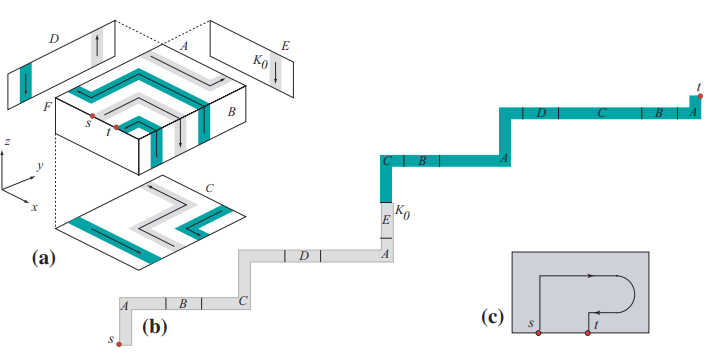
\includegraphics[width=\textwidth]{./figs/New_diagram_who_dis.png}
    \begin{center}
      \footnotesize \textbf{Figure}: \textbf{(a)} is a spiral path and \textbf{(b)} is its unfolding.
    We will use diagrams such as \textbf{(c)} as shorthand \footfullcite[Fig. 3]{Damian_Flatland_Orourke}
    \end{center}
  \end{frame}

  \begin{frame}{Recursive step spiral path when all ends are trivial}
    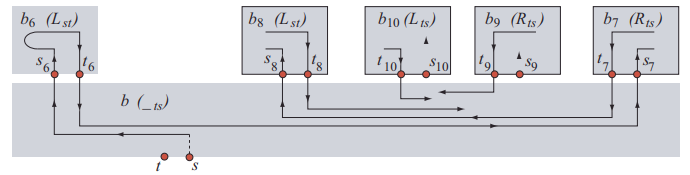
\includegraphics[width=\textwidth]{./figs/Recursive_step_example_front.png}
    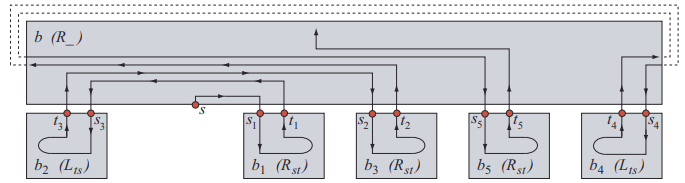
\includegraphics[width=\textwidth]{./figs/Recursive_step_example_back.png}
   
    \begin{center}
      \tiny
      \textbf{Figure}:
      Given an initial ``direction'' (left or right), we travel this direction until we see a front child, which we traverse to, then exit and move the opposite direction;
      we do this until we finish the children, circle around the band, and execute a similar process on the back children.
      After the last one, we double back.
      We employ a familiar gadget for the back face if there are no back children.
      \footfullcite[Fig. 4,5]{Damian_Flatland_Orourke}
    \end{center}
  \end{frame}

  \begin{frame}{Recursive step spiral path when all ends are trivial}
    \begin{columns}
      \begin{column}{.5\textwidth}
        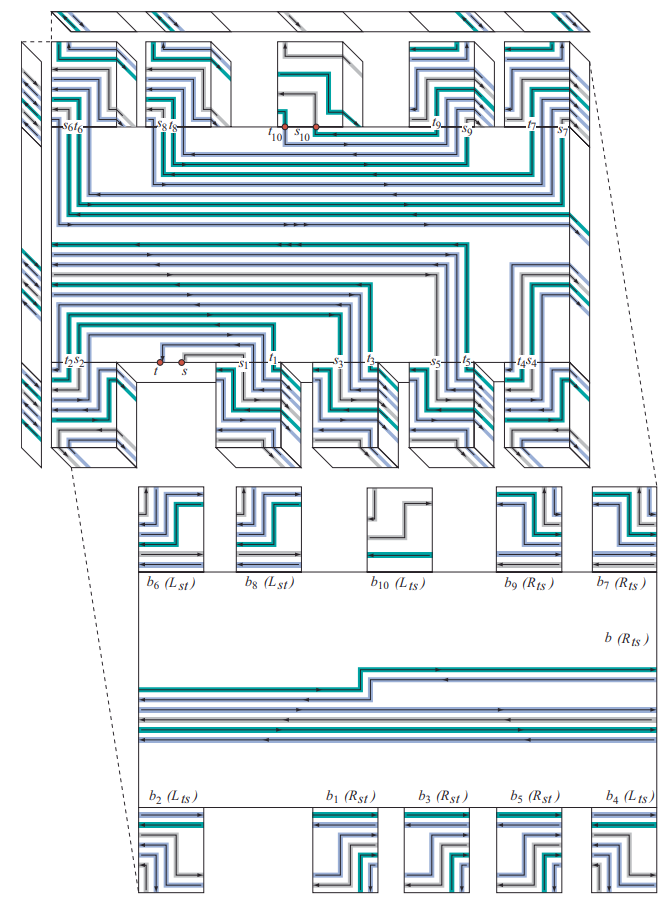
\includegraphics[height=.8\textheight]{./figs/Recursive_step_example_capped.png}
      \end{column}
      \begin{column}{.5\textwidth}
        \footnotesize \textbf{Figure}: a full picture of the spiral path in the previous example.
        \footnote[frame]{\fullcite[Fig. 6]{Damian_Flatland_Orourke}}
        We henceforth refrain from showing full examples.\\
        \;\\
        \pause Note that ``doubling back'' creates many paths on the middle band.
        This has a ``path density'' of $4n - 2$, where $n$ is the number of children.\\
        \;\\
        \pause We might have to ``double back'' many times for deep unfolding trees, which will double the path density each time.
        This yields an upper bound of $2^{O(n)} \times 2^{O(n)}$ refinement in general.
      \end{column}
    \end{columns}
  \end{frame}

  \begin{frame}{More complicated recursive example}
    \begin{center}
      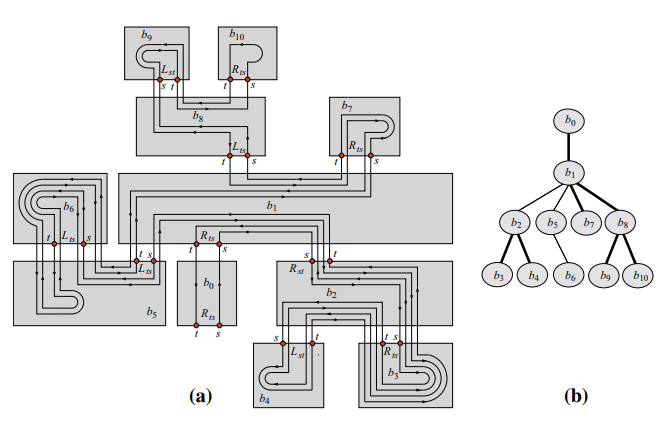
\includegraphics[width=.9\textwidth]{./figs/Example_with_much_doubling.png}\\
      \tiny \textbf{Figure}: another example, with \textbf{(a)} the unfolding and \textbf{(b)} the unfolding tree. 
      Note that the path is ``quadrupled'' on certain children of high depth.\footfullcite[Fig. 7]{Damian_Flatland_Orourke}
    \end{center}  
  \end{frame}

  \begin{frame}{Path density of the epsilon-unfolding strategy}
    We can construct high depth trees which lead to high path density.
    The following example shows that we get $2^{\Omega(n)}$ path density, and hence $2^{\Omega(n)} \times 2^{\Omega(n)}$ refinement.
    
    \;\\

    \begin{center}
      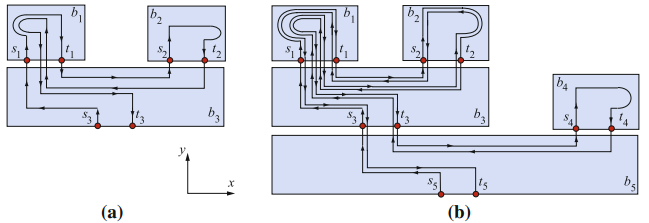
\includegraphics[width=\textwidth]{./figs/Exponential_path_density.png}\\
      \tiny \textbf{Figure}: \textbf{(a)} has path density 4, \textbf{(b)} has 8, and in general this pattern yields an $n$ box polyhedron with path density $2^{\lfloor n/2 \rfloor}$.\footfullcite[Fig. 7]{Damian_Demaine_Flatland}
    \end{center}
  \end{frame}

  \begin{frame}{Improvements: the delta-unfolding strategy}
    There have been multiple improvements on epsilon-unfolding which use the same basic strategy.
    The first is the \emph{delta-unfolding strategy}, due to \footfullcite{Damian_Demaine_Flatland}:
    define a node in the unfolding tree to be \emph{heavy} if it spans a subtree containing at least half of the children of the parent.
    Traverse heavy children last.
    
    \pause Path density is related to the number of times the spiral path ``visits a child of a band.''
    We guarantee that heavy children are visited once,
  \end{frame}

\begin{frame}{Illustration of the delta-unfolding: heavy back child}
  \begin{center}
    \includegraphics[width=\textwidth]{./figs/Delta_unfolding_back.png}\\
    \tiny \textbf{Figure}: It's easy to visit heavy back children last: simply choose the correct first back child to visit, which one may choose arbitrarily.\footfullcite[Fig. 10]{Damian_Demaine_Flatland}
  \end{center}
\end{frame}

\begin{frame}{Illustration of the delta-unfolding: heavy front child}
  \begin{center}
    \includegraphics[width=.75\textwidth]{./figs/Delta_unfolding_front.png}\\
    \tiny \textbf{Figure}: in the case of a back child, we'll actually have to visit non-heavy children four times via the above strategy.\footfullcite[Fig. 9]{Damian_Demaine_Flatland}
  \end{center}
\end{frame}

\begin{frame}{Sketch of asymptotics}
  Let $b$ be a band, and let $b_1,\dots,b_{n(b)}$ be the children of $b$.
  Suppose $b_{\text{heavy}}$ is the heavy child of $b$ if one exists.
  Write $R(n(b))$ for the asymptotic upper bound for the path density at $b$.
  Then, there are at most $O(n(b))$ segments on $b$'s top face, so we have
  \begin{align*}
    R(n(b)) 
    &= \max \left\{ O(n(b)), 4 \max_{i \text{ non-heavy}} R(n(b_i)), R(n(b_{\text{heavy}}))\right\}\\
    &\leq \max \left\{ O(n(b)), 4 \max_{i \text{ non-heavy}} R\left( \frac{n(b)}{2} \right), R(n(b) - 1)\right\}\\
    &\leq \max \left\{ O(n(b)), 4 R\left( \frac{n(b)}{2} \right), R(n(b) - 1))\right\}
  \end{align*}
  This leads to $R(n(b)) = O(n^2)$.
  This can be shown to be sharp using polyhedron forming a full binary tree.
\end{frame}
  
\begin{frame}{Linear unfolding}
  We can do better:
  in fact, we can get linear refinement \footfullcite{Damian_Demaine}.

  Instead of \emph{top down} construction of \emph{one spiral path}, we do the following, where $T(b)$ denotes the subtree spanned by band $b$.

  Inducting on increasing height of $T(b)$, we construct one spiral path with endpoints on the front rim of $b$ per leaf node in $T(b)$, such that:
    \begin{itemize}
      \item the endpoints of each spiral path are adjacent,
      \item no two paths cross, and
      \item all bands in the subtree spanned by $b$ have been spiraled around at least once.
    \end{itemize}
  We then use a gadget on the root node to stitch these into one path.
\end{frame}

\begin{frame}{Linear unfolding example}
  \begin{columns}
    \begin{column}{.7\textwidth}
      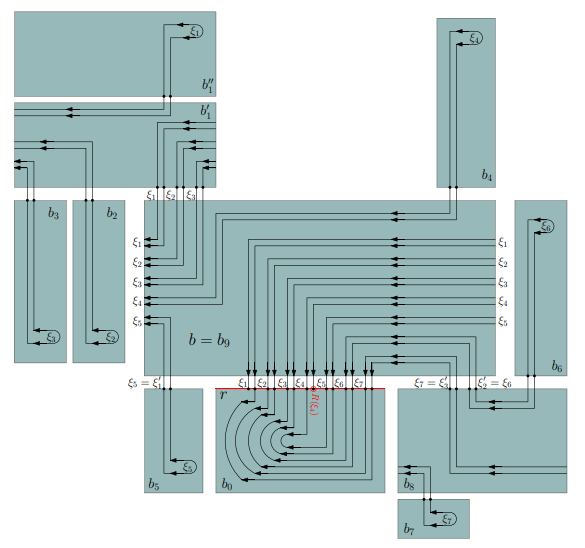
\includegraphics[height=.8\textheight]{./figs/Linear_unfolding.png}
    \end{column}
    \begin{column}{.3\textwidth}
      \footnotesize \textbf{Figure}: an example of the linear unfolding strategy.
      \footnote[frame]{\fullcite[Fig. 4]{Damian_Demaine}}\\
      \;\\
      The directions indicated on paths correspond with the direction of the unfolding tree.\\
      \;\\
      Note that layers don't ``double'' the path density; instead, they add $O(1)$ to the path density!
    \end{column}
  \end{columns}
\end{frame}

\begin{frame}{Linear unfolding 2}
  The above strategy explains how to work with root node having one child, and internal nodes having both front and back children;
  we can guarantee this by only adding $O(1)$ cleverly placed cuts.

  \pause From the above handwave, we require $O(n) \times O(n)$ refinement.
  
  \pause This is sharp:
  take an orthogonal polyhedron with $O(n)$ root nodes.
\end{frame}

\begin{frame}{Sketch of genus $g \leq 2$ generalization}
  We were secretly using three (perhaps nonobvious) facts of genus 0 orthogonal polyhedra $P$:
  \begin{enumerate}
    \pause \item The unfolding tree of $P$ is acyclic (i.e. it \emph{is} a tree).
    \pause \item There is a band with a rim enclosing a face of $P$ which can be chosen to be a root node.
    \pause \item The back rim of each leaf node encloses a face of $P$.
  \end{enumerate}
  \pause To fix the first, we replace the first tree with a \emph{rim unfolding graph}, and work with a spanning tree of that graph, called a \emph{rim spanning tree.}
\end{frame}

\begin{frame}{Fixes to our problems with genus $g \leq 2$}
  Suppose the genus of $P$ is $g \leq 2$.
  \pause 
  \begin{lemma}
    There is an orientation of $P$ such that it has a face rim which may be chosen as a root node.
  \end{lemma}
  \pause
  \begin{lemma}
    There are at most $g$ leaves with back rims not enclosing a face. 
  \end{lemma}
  \pause We just need a gadget that deals with at most 2 nonface leaf nodes!
  They provide one in \footfullcite{Damian_Demaine}.

  This gives grid unfolding with linear refinement for genus $g \leq 2$.
\end{frame}

\end{document}

